\documentclass{article}
\usepackage{fullpage}
\usepackage{subfiles}

\usepackage{epsfig}
\usepackage{amsfonts}
\usepackage{amssymb}
\usepackage{amstext}
\usepackage{amscd}
\usepackage{amsmath}
\usepackage{amsthm}
\usepackage{times}
\usepackage{graphicx}
\usepackage{alltt}
\usepackage{hyperref}
\hypersetup{
    colorlinks=true,
    citecolor=red,
    filecolor=black,
    linkcolor=blue,
    urlcolor=blue
}

\usepackage{float}
\usepackage{tikz}
\usetikzlibrary{arrows.meta, shapes.geometric, calc, shadows, decorations.pathreplacing, shapes.misc, math,calc} %tikz stuff

\newtheorem{claim}{Claim}

\usepackage[linesnumbered,lined,boxed,commentsnumbered,ruled,vlined]{algorithm2e}
\usepackage{enumerate}

\begin{document}

\noindent
\fbox{
\parbox{\textwidth}{
\begin{Large}
{\bf CS 577: Introduction to Algorithms\hfill Greedy Review problems solutions}
\end{Large}
}}

\section*{Problem 1}
\begin{enumerate}[a)]
	\item Let $G'=(V,E')$ be a subgraph of $G$. We will prove each direction of the argument separately:

		\begin{itemize}
				\item $G'\subset G$ is obtained by taking a spanning tree $T$
and adding one edge $e$ $\Rightarrow$ $G'$ is special.\\
 Since $T$ is a spanning tree, it is connected and contains no cycle. Then
adding the edge $e$ into $T$ will form exactly one cycle and therefore $G'$ is
\emph{special}. 

				\item $G'$ is special $\Rightarrow$ is obtained by taking a
spanning tree $T$ and adding one edge $e$.\\
Since $G'$ is \emph{special}, then it is connected and contains exactly
one cycle. Pick an arbitrary edge $e$ in this cycle and delete it from $G$, we
obtain a new graph $G_1$. Since $G_1$ is still connected and contains no cycle,
$G_1$ is a spanning tree of $G$.
			\end{itemize}

	\item Using  what we know from the previous question, we need to take a
spanning tree and add an edge in order to obtain a special subgraph $G'$. Since
we want a minimum weight $G'$ we will find a minimum spanning
tree (and not \emph{any}) spanning tree, and select an edge of minimum weight
(from those that are not selected for the MST) to add. This algorithm needs
$O(m\log m)$ to find a MST (using Kruskal's algorithm for example) and an
additional $O(m)$, so in total $O(m\log m)$.\\

In order to prove correctness for this algorithm, we will show that for any
arbitrary special graph $F$ our solution $G'$ gives a graph with less weight.
Since $F$ is a special subgraph, we know that $F$ is connected and contains
exactly one cycle $C$. Let $f$ be the edge with maximum weight in cycle $C$.
From the proof of part (a), we have $F=T'\cup\{f\}$, where $T'$ is a spanning
tree of $G$.  But, since $T$ is an MST, the weight of $T$ is no larger than the
weight of $T'$.  Meanwhile, since $f$ has the maximum weight in the cycle $C$,
we know that $f\notin T$ by the ``cycle property''. Therefore by our choice of
edge $e$ in the algorithm, we have $w_e\le w_f$. Finally, we get
$w_{G'}=w_T+w_{e}\le w_{T'}+w_{f}=w_{F}$, as claimed. This implies that our
algorithm successfully returns a minimum-weight special subgraph of $G$.
\end{enumerate}

\section*{Problem 2}
In the classic setting for the minimum spanning tree all edges have constant
weights over time, so we were able to sort them in a unique way. Then we could
choose the minimum weight ones to include in the minimum spanning tree. The
difference here is that over time this sorting changes, so the edges that were
of minimum weight at time $t_1$ may not me minimum at time $t_2 > t_1$. 

The idea for this problem is to find time intervals that this sorting remains
constant. In other words, we want to divide $[l,r]$ into subintervals where there
are no changes in this sorting. This means that no two functions of weights
$f_i$ and $f_j$ that are $f_i<f_j$ in this interval will swap and become
$f_i>f_j$. 

The key observation here is that all functions are monotone, so -in
the worst case- each one will "change" relative position with each other at
most 1 time in any given interval. Think that the equation $f_j = f_i
\Leftrightarrow a_it+b_i = a_jt+b_j$ has a unique solution.

So, by solving these equations for all pairs of edges (so ${m\choose 2} = O(m^2)$
equations) we find the times that something in the sorting changes, so in the
intervals between these $t_i$'s, the sorting is constant and we can run any
algorithm that calculates an MST.

The algorithm looks like this:

\begin{algorithm}[H]
\KwData{Graph $G(V,E)$, functions $f_e = a_et+b_e$ $\forall e\in E$}
Solve equation $f_i=f_j$ for each pair $i,j\in E$\;
Sort solutions $t_{ij}$ in increasing order\;
Discard all $t_i > r$ and $t_i < l$\;
\ForEach{interval $[t_i, t_j]$}{
	Run Kruskal with edges cost $f_j(t_i)$\;
	$c_i$ =  MST cost\;
}
\Return $\min c_i$\;
\caption{Algorithm Problem 2}
\end{algorithm}

The algorithm will take $O(m^3 \ log n)$ time; the time to solve the $m^2$
equations is $O(m^2)$, and for each of the $m^2$ (in the worst case) intervals
we run Kruskal's algorithm so in total $O(m^2 m \log n) =  O(m^3\log n)$ time.

\section*{Problem 3}

\begin{enumerate}
	\item The width of a spanning tree is the edge of maximum width. If we
could remove all edges with weight above $W$ and the graph remained connected,
then we would be able to find a spanning tree with width at most $W$. We can
use any graph traversal algorithm (like BFS or DFS), and each time we find an
edge with weight $>W$, we would delete it. Then, we run again the same
algorithm on the graph that remained, in order to see if it is connected (so if
we were able to reach each node from the initial one).  If the answer to this
is yes, then we know there exists a spanning tree with width at most $W$.

The running time of this algorithm is linear on the input, since we just run
BFS or DFS twice, so each time with cost $V+E$. Therefore in total $O(V+E)$.

	\item For this question we will see two different solutions. One with
complexity based on the maxomum weight, and one with complexity based only on
$m$ and $n$.Lets denote $\operatorname{Alg}(W)$ the algorithm of the previous question, which
takes as argument the weight $W$ and replies ``Yes'' if there exists a spanning
tree with weight $<W$ and ``No'' otherwise. \\

\textbf{Solution 1:}\\
 We would like to do binary search to the values of $W$ in order to find the
smaller $W$ for which we can find a spanning tree. In order to do that, we need
an interval in which we will run the binary search. Since the weights are
finite, we will just find the maximum weight of an edge in the graph, by
traversing it once (so using BFS for example).

\begin{algorithm}
\KwData{Graph $G(V,E)$}
Find $W_{max}$\;
$h\leftarrow W_{max}$\;
$l\leftarrow 0$\;
\While{$l<h$}{
	$m \leftarrow \frac{l+h}{2}$\;
	\If{$Alg(m)$ is "Yes"}{
		$h\leftarrow m$\;
	}
	\Else{
		$l\leftarrow m$\;
	}
}
\Return m\;
\caption{Algorithm Problem 3}
\end{algorithm}

This algorithm initially makes $O(V+E)$ time to find $W_{max}$ by traversing
the graph once (using BFS for example). Then it requires $O(\log W_{max}
(V+E))$ steps to do the binary search, where in each of the $\log W_{max}$
iterations it will run $\operatorname{Alg}(W)$ once, which requires $O(V+E)$,
so in total $O(\log W_{max}(V+E))$

\textbf{Solution 2:}\\
In this solution, in order to avoid including $W_{max}$ in the runtime of the
algorithm, we can think of something slightly different. The main observation
we use in order to avoid this is that $W_{max}$ can be very large, but not all
distinct values $\{0, 1,\dots, W_{max}\}$ appear as edge weights, but only $m$
of them. So instead of doing binary search in the different weights, we will do
binary search in the weight values that actually appear on the graph, so by
sorting the edges by weight.

\begin{algorithm}
\KwData{Graph $G(V,E)$, $|E|=m,\ |V|=n$}
Sort edges by weight and store them in array $M$\;
$h\leftarrow m-1$\;
$l\leftarrow 0$\;
\While{$l<h$}{
	$temp \leftarrow \frac{l+h}{2}$\;
	\If{$Alg(M[temp])$ is "Yes"}{
		$h\leftarrow temp$\;
	}
	\Else{
		$l\leftarrow temp$\;
	}
}
\Return $M[temp]$\;
\caption{Alternative algorithm for Problem 3}
\end{algorithm}

This algorithm initially makes $O(m\log m)$ time to sort the edges, and then it
requires $O(\log m \cdot (V+E))$, so in total $O(m\log m)$

	\end{enumerate}

\section*{Problem 4}
This problem is a simple modification of Dijkstra's algorithm. Remember that in
order to find a shortest path from $s$ to $t$, Dijkstra's algorithm starts by
assuming all nodes are at infinite distance from the starting node $s$, and
then proceeds by trying to find each time the edge that gives us the shortest
path to a new node. Would Dijkstra's algorithm work in this case? The answer is
no, and it is easy to see, with a simple example, that the shortest path does
not necessarily imply minimum bottleneck length between two nodes. In the
example below, the shortest path uses node $u_1$ and has length but bottleneck
distance $5$, while the path using nodes $u_2, u_3$ has length $7$ but
bottleneck distance 3.

\begin{figure}[H]
\centering
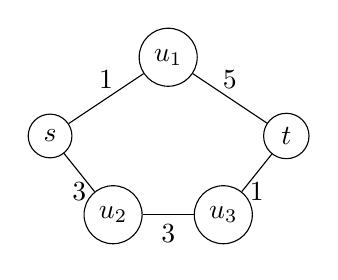
\begin{tikzpicture}
\node[shape=circle,draw=black] (A) at (0,0) {$s$};
\node[shape=circle,draw=black] (U1) at (1.5,1) {$u_1$};
\node[shape=circle,draw=black] (U2) at (0.8,-1) {$u_2$};
\node[shape=circle,draw=black] (U3) at (2.2,-1) {$u_3$};
\node[shape=circle,draw=black] (T) at (3,0) {$t$};

\draw[-] (A)-- node[above] {$1$} ++ (U1);
\draw[-] (A)-- node[below] {$3$} ++  (U2);
\draw[-] (U1)-- node[above] {$5$} ++ (T);
\draw[-] (U2)-- node[below] {$3$} ++ (U3);
\draw[-] (U3)-- node[below] {$1$} ++ (T);

\end{tikzpicture}

	\caption{Counterexample for Dijkstra's}
	\label{fig:counterexample}
	\end{figure}

The real problem with Dijkstra is that it only looks at the total distance, and
not at the maximum edge when considering the next one, and this is precisely
what we need to change in order for our algorithm to work. So instead of
keeping track of the tentative distance $d'(v)$ from the source $s$, we replace
this by the maximum edge in the path so far. So in line 5 of the algorithm
\ref{algo:dijkstra} below, we are essentially saying that when considering node
$v$, we can either reach it via $tmp$, in which case the maximum length is
$\max \{d(tmp), w(tmp,v)\}$ (maximum until tmp compared to the distance $w(v,
tmp)$) or we can reach it via another path with maximum length $d(v)$.

Since we need to find the
bottleneck distance for every two nodes, we will start from node $s$ and run it
for all pairs $(s,i),\ \in V$, then for the next node, we will run it for all
pairs except $(u,s)$ etc. Since we have $O(n)$ such pairs, the running time
will be $n^2$ times the running time of Dijkstra, so $O(n^2m\log n)$ in total.


\begin{algorithm}
\KwData{Graph $G(V,E)$, starting node $s$, target node $t$}
Initialize Priority Queue: $d(v)=\infty,\ \forall v\in \{V\setminus s\}, d(s)=0$\;
\While{PQ $\neq \emptyset$}{
	tmp $\leftarrow$ pop(PQ)\;
	\ForEach{$v$ neighbor of tmp}{
		$d'(v) \leftarrow \min\{ d(v), \max \{d(tmp), w(v,tmp)\} \}$\;		
	}
}
\Return $d(t)$\;
\caption{Modification of Dijkstra}
\label{algo:dijkstra}
\end{algorithm}


\end{document}

